\chapter{Das Flächenmaß auf Untermannigfaltigkeiten}
  \sidenote{Vorlesung 21}{25.01.2021}

  \begin{definition}
    Sei $\script{U} \subseteq \mathbb{R}^n$ offen. Eine Abbildung $f \in C^1(\script{U}, \mathbb{R}^{n+k})$ heißt \textbf{Immersion}, wenn gilt:
    $$Rang \ Df(x) = n \Leftrightarrow Ker \ Df(x) = \{0\} \ \forall \ x \in \script{U}$$
    $\frac{\partial f}{\partial x_1}(x), ..., \frac{\partial f}{\partial x_n}(x)$ bilden eine Basis von $Bild \ Df(x) \subseteq \mathbb{R}^{n+k}$. $n$ heißt \textbf{Dimension}, $k$ die \textbf{Kodimension} von $f$.\\
    Wir definieren die \textbf{Gramsche Matrix} oder \textbf{induzierte Metrik}
    $$g(x) = Df(x)^{\top} Df(x)$$ 
    $$\text{bzw. } g_{ij}(x) = <\frac{\partial f}{\partial x_i}|x|, \frac{\partial f}{\partial x_j}|x|>$$
    $\rightarrow (g_{ij})$ ist für $f \in C^1(\script{U}, \mathbb{R}^{n+k})$ beliebig definiert und positiv semidefinit.\\
    Die Matrix ist genau dann strikt positiv definit und damit invertierbar, wenn $f$ eine Immersion ist:
    $$<g(x)v, v> = |Df(x)v|^2 \geq 0$$
    $$\implies Ker \ g(x) = Ker \ Df(x)$$
  \end{definition}

  \begin{definition}{Flächenformel}
    $\script{U} \subseteq \mathbb{R}^n$ offen, $f \in C^1(\script{U}, \mathbb{R}^{n+k})$ eine $n$-dimensionale Immersion mit Gramscher Matrix $g$, und $E \subseteq \script{U}$ sei $\lambda^n$-messbar.\\
    Der ($n$-dimensionale) \textbf{Flächeninhalt} von $f$ auf $E$ ist definiert durch
    $$A(f,E) = \int\limits_E Jf(x) \ dx$$
    $$\text{mit } Jf = \sqrt{det \ g}$$
    $Jf$ heißt \textbf{Jacobische} von $f$.
  \end{definition}

  \newpage
  \begin{example}
    \begin{enumerate}
      \item[]
      \item $f = S \circ \Phi: \script{U} \to \mathbb{R}^{n+k}, \Phi \in C^1(\script{U}, \script{V})$ Diffeomorphismus zwischen $\script{U}, \script{V} \subseteq \mathbb{R}^n$ offen und $S: \mathbb{R}^n \to Y \subseteq \mathbb{R}^{n+k}$ lineare Isometrie, $E \subseteq \script{U}$ messbar, $Df(x) = S \ D\Phi(x)$
        \begin{align*}
          \implies A(f,E) 
          &= \int\limits_E \sqrt{det \ D\Phi(x)^{\top} S^{\top} S D\Phi(x)} dx\\
          &= \int\limits_E |det \ D\Phi(x)| dx \stackrel{Trafo}{=} \lambda^n(\Phi(E))
        \end{align*}
      \item 1-dim Immersion $f: I = (a,b) \to \mathbb{R}^n \ f=f(A)$ heißt \textbf{reguläre Kurve} Gramscher Matrix $g_{11}=<f'(A), f'(A)> = ||f'(A)||^2$\\
        Länge von Kurve $\rightarrow L(f) = \int\limits_a^b ||f'(A)|| dt$\\
        $$f(A) = (cos(t), sin(t)) \ \ \ L(f, [0, 3\pi]) = 3\pi$$
      \item 2-dim Immersion in $\mathbb{R}^n \ (n=2, k=1) \ f:\script{U}\to\mathbb{R}^3, f=f(x,y)$ heißt \textbf{reguläre Fläche}
        $$(g_{ij}) = \begin{pmatrix}
          ||\frac{\partial f}{\partial x}||^2 & <\frac{\partial f}{\partial x}, \frac{\partial f}{\partial y}>\\
          <\frac{\partial f}{\partial x}, \frac{\partial f}{\partial y}> & ||\frac{\partial f}{\partial y}||^2
        \end{pmatrix}$$ 
        $\implies Jf = \sqrt{||\frac{\partial f}{\partial x}||^2 ||\frac{\partial f}{\partial y}||^2 - <\frac{\partial f}{\partial x}, \frac{\partial f}{\partial y}>^2} = ||\frac{\partial f}{\partial x} \times \frac{\partial f}{\partial y}||$\\
        $(||a||^2||b||^2-<a,b>^2 = ||a \times b||^2 \text{ siehe LA})$\\
        \begin{align*}
          &\text{Polarkoordinaten:}\\
          &f: \script{U} = (0, \pi) \times (0, 2\pi) \to S^2\subseteq \mathbb{R}^3\\
          &f(\theta, \phi) = \begin{pmatrix}
            sin(\theta)cos(\phi) & sin(\theta)sin(\phi) & cos(\theta)
          \end{pmatrix}\\
          &\stackrel{\text{Kap. VII}}{\implies} Jf(\theta, \phi) = sin(\theta) \implies f \text{ reguläre Fläche}\\
          &A(f) = \int\limits_0^{\pi}\int\limits_0^{2\pi} sin(\theta) \ d\phi \ d\theta = 4\pi
        \end{align*}
      \item siehe Aufschrieb
    \end{enumerate}
  \end{example}

  \begin{theorem}
    $\Phi \in C^1(\script{U}, \script{V})$ Diffeomorphismus, $\script{U}, \script{V} \subseteq \mathbb{R}^n$ offen und $f \in C^1(\script{V}, \mathbb{R}^{n+k})$ Immersion. Dann gilt:
    $$A(f, \Phi(E)) = A(f\circ\Phi, E) \ \ \ \forall \ E \subseteq \script{U} \ \lambda^n\text{-messbar}$$
  \end{theorem}
  \begin{proof}
    siehe Aufschrieb
  \end{proof}

  \begin{definition}[Untermannigfaltigkeiten]
    Eine Menge $M \subseteq \mathbb{R}^{n+k}$ heißt \textbf{Untermannigfaltigkeit} des $\mathbb{R}^{n+k}$, der Klasse $C^r,\\ r\in \mathbb{N}\cup\{\infty\}$ offen (mit $M \in \Omega$) und $\exists \ \Phi: \Omega \to \Phi(\Omega) \\
    C^r$-Diffeomorphismus mit
    $$\Phi(M \cap \Omega) = (\mathbb{R}^n \times \{0\}) \cap \Phi(\Omega)$$
    ($\Phi$ heißt \textbf{lokale Plättung} von $M$)\\
    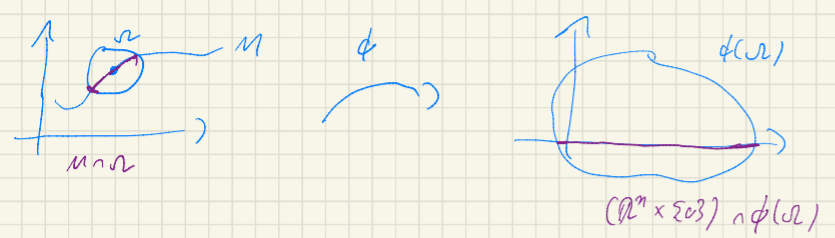
\includegraphics[width=\textwidth]{img/VIII_4_UnterMGF.png}
  \end{definition}

  \begin{theorem}
    Sei $M \subseteq \mathbb{R}^{n+k}$. Dann sind äquivalent:
    \begin{enumerate}
      \item $M$ ist $n$-dimensionale Untermannigfaltigkeit der Klasse $C^r$
      \item $\forall p \in M \ \exists \ \Omega\subseteq\mathbb{R}^{n+k}$ offene Umgebung vvon $p$ und $f \in C^r(\Omega, \mathbb{R}^k)$ mit $M \cap \Omega = f^{-1}(0)$ und $Rang \ Df = k$ auf $\Omega$
      \item $\forall p \in M \ \exists$ offene Umgebungen $\script{U}\subseteq \mathbb{R}^n, V\subseteq \mathbb{R}^k$ und $g \in C^r(\script{U}, \script{V})$, so dass nach geeigneter Permutation der Koordinaten gilt:\\
      $$M \cap (\script{U} \times \script{V}) = \{(x, g(x)) \ | \ x \in \script{U}\}$$
      \item $\forall p \in M \ \exists$ offene Umgebung $\script{U}\subseteq \mathbb{R}^n$ und $\script{C} \in C^r(\script{U}, \mathbb{R}^{n+k})$ mit $\script{C}(x_0) = p$ für ein $x_0 \in \script{U}$ und $Rang \ D\script{C}(x) = n \ \forall \ x\in M$, so dass $\script{C}$ offene Teilmengen von $\script{U}$ in relativ offene Teilmengen von $M$ abbildet. 
    \end{enumerate}
  \end{theorem}

  \sidenote{Vorlesung 22}{29.01.2021}

  \begin{theorem}
    Jede $n$-dimensionale Untermannigfaltigkeit $M \subseteq \mathbb{R}^{n+k}$ ist als abzählbare Vereinigung $M = \bigcup\limits_{i\in\mathbb{N}} K_i$ von kompakten Mengen darstellbar.
  \end{theorem}
  \begin{proof}
    siehe Aufschrieb
  \end{proof}

  \begin{definition}
    Sei $M \subseteq \mathbb{R}^{n+k}$ eine $n$-dimensionale Untermannigfaltigkeit der Klasse $C^1$. Eine \textbf{lokale Parametrisierung} von $M$ ist eine injektive Immersion $f: \script{U} \to M \subseteq \mathbb{R}^{n+k}$, wobei $M \subseteq \mathbb{R}^n$ offen und $f \in C^1$.
  \end{definition}

  \begin{lemma}
    Für jede Untermannigfaltigkeit $M \subseteq \mathbb{R}^{n+k}$ der Klasse $C^1$ gibt es lokale\\
    $C^1$-Parametrisierungen $f_i:\script{U}_i \to M$, wobei $i\in\mathbb{N}$, sodass $M = \bigcup\limits_{i \in \mathbb{N}} f_i(\script{U}_i)$
  \end{lemma}
  \begin{proof}
    siehe Aufschrieb
  \end{proof}

  \begin{theorem}
    $M \subseteq \mathbb{R}^{n+k}$ $C^1$-Untermannigfaltigkeit. Dann gelten:
    \begin{enumerate}
      \item Ist $f: \script{U} \to M$ lokale Parametrisierung von $M$, so ist $f(\script{U})$ offen in $M$ und $f: \script{U} \to f(\script{U})$ ist homeomorph, d.h. $f^{-1}$ ist stetig bzgl. euklidischer Metrik auf $f(\script{U})$.
      \item Sind $f_i:\script{U}_i \to f(\script{U}_i) = \script{V}_i$ für $i = 1,2$ lokale $C^1$-Parametrisierung von $M$, so ist $f_2^{-1}\circ f_1: f_1^{-1}(\script{V}_1\cap\script{V}_2) \to f_2^{-1}(\script{V}_1\cap\script{V}_2)$ ein $C^1$-Diffeomorphismus. 
    \end{enumerate}
  \end{theorem}
  \begin{proof}
    siehe Aufschrieb
  \end{proof}

  \begin{theorem}[Flächenmaß]
    $M \subseteq \mathbb{R}^{n+k} C^1$-Untermannigfaltigkeit. Dann heißt $E \subseteq M$ messbar, falls gilt:
    $$f^{-1}(E) \text{ ist } \lambda^n\text{-messbar für jede lokale Parametrisierung } f: \script{U} \to M$$
    Das System $\script{M}$ der messbaren Teilmengen von $M$ ist eine $\sigma$-Algebra. Diese enthält die Borelmengen in $M$. Weiter gibt es genau ein Maß $\mu_M$ auf $\script{M}$, so dass für jede lokale Parametrisierung $f: \script{U} \to M$ und jedes $E \subseteq f(\script{U})$ messbar gilt:
    $$\mu_M(E) = \int\limits_{f^{-1}(E)}Jf(x) \ dx$$
  \end{theorem}
  \begin{proof}
    siehe Aufschrieb
  \end{proof}

  \newpage
  \begin{theorem}[Oberflächenintegral]
    Sei $M \subseteq \mathbb{R}^{n+k} n$-dimensionale $C^1$-Untermannigfaltigkeit und $M = \bigcup\limits_{i \in \mathbb{N}} M_i$ eine paarweiße disjunkte, messbare Zerlegung mit $M_i \subseteq \script{V}_i$ für lokale Parametrisierungen $f_i: \script{U}_i \to \script{V}_i$. Für eine messbare Funktion $u: M \to \bar{\mathbb{R}}$ gilt:
    $$\int\limits_M u \ d\mu_M = \sum\limits_{i \in \mathbb{N}} \int\limits_{f_i^{-1}(M_i)} u(f_i(x))\ Jf_i(x)\ dx$$
  \end{theorem}

  \sidenote{Vorlesung 23}{01.02.2021}
  \begin{lemma}
    Sei $T:\mathbb{R}^{n+k} \to \mathbb{R}^{n+k}$ eine \textbf{Ähnlichkeitsabbildung}, d.h. $\exists \lambda>0, Q\in O(n+k)$ und $a\in\mathbb{R}^{n+k}$ mit $T(p) = \lambda Q(p+a)$. Ist $M \subseteq \mathbb{R}^{n+k}$ eine $n$-dimensionale $C^1$-Untermannigfaltigkeit, so auch $N = T(M)$ und für $\mu_M$ bzw. $\mu_N$ gilt:
    \begin{enumerate}
      \item Ist $A \subseteq M$ messbar $\implies T(A) \subseteq N$ messbar und 
        $$\mu_N(T(A)) = \lambda^n (\mu_M(A))$$
      \item Ist $u: N \to \bar{\mathbb{R}} \ \mu_N$-messbar, so ist $u \circ T: M \to \bar{\mathbb{R}} \ \mu_M$-messbar und es gilt, sofern eines der Integrale existiert:
        $$\int\limits_N u(q) \ d\mu_N(q) = \lambda^n \int\limits_M u(T(p)) \ d\mu_M(p)$$
    \end{enumerate}
  \end{lemma}
  \begin{proof}
    siehe Aufschrieb
  \end{proof}

  \begin{theorem}[Zwiebelformel]
    Für $u \in L^1(\mathbb{R}^{n+1})$ ist $u|_{\partial B_r(0)} \subseteq L^1(\mu_{\partial B_r(0)})$ für fast alle $r>0$ und es gilt:
    \begin{align*}
      \int\limits_{\mathbb{R}^{n+1}} u(p) \ dp
      &= \int\limits_0^{\infty} \int\limits_{\partial B_r(0)} u(p) \ d\mu_{\partial B_r(0)}(p)\ dr\\
      &= \int\limits_0^{\infty} r^n \int\limits_{S^n} u(rw) \ d\mu_{S^n}(w)\ dr
    \end{align*}
  \end{theorem}
  \begin{proof}
    siehe Aufschrieb
  \end{proof}

  \newpage
  \begin{example}
    Mit $u = \psi_{B_1(0)}$ folgt für $w_n = \mu_{S^n}(S^n)$:
    $$\alpha_{n+1} = \lambda^{n+1}(B_1(0)) = \int\limits_0^1 \mu_{\partial B_r(0)} (\partial B_r(0)) \ dr = \int\limits_0^1 w_n r^n \ dr = \frac{w_n}{n+1}$$
    $\implies w_n = (n+1) \alpha_{n+1}$\\
    z.B. $w_1 = 2\pi, w_2 = 4\pi, w_3 = 2\pi^2, ...$
  \end{example}